\section{周期信号的傅里叶级数型}

本节简单介绍周期信号的傅里叶级数,具体推导参见《微积分笔记》。

本节要点:
\begin{itemize}
    \item 掌握傅里叶级数的三角级数形式;
    \item 掌握傅里叶级数的复指数形式;
    \item 理解傅里叶级数的量纲;
    \item 熟练掌握周期信号的复指数展开。
\end{itemize}

%============================================================
\subsection{三角级数展开}

{\bf 三角级数展开}:当周期为$T$的信号$x\left( t \right) $满足狄利克雷收敛条件时,其在周期内可以展开成三角级数,即无穷项余弦函数的叠加,且收敛于该周期信号:
\[
x\left( t \right) =A_0+\sum_{n=1}^{+\infty}{A_n\cos \left( \omega _nt+\varphi _n \right)}
\]
\begin{itemize}
    \item $A_0,A_n$:{\bf 傅里叶系数},$A_0$表示信号的{\bf 直流分量}或{\bf 基频分量};
    \item $\omega _n=n\omega _0$:对应余弦项的{\bf 角频},称$\omega _0=2\pi /T$为{\bf 基频};
    \item $\varphi _n$:对应余弦项的{\bf 初始相位},简称{\bf 相位}。
\end{itemize}

数学上,周期函数都能展开成三角级数,但不一定收敛,即便收敛也不一定收敛至原函数。
如果周期函数满足狄利克雷充分条件,即周期函数必须在一个包含原点的最小周期内连续,或只有有限个一类间断点,而且只有有限个极值点,则三角级数收敛在原函数。
这样的三角级数称为傅里叶级数。

周期信号展开成三角级数后,对信号又多了一种描述方法,即以频率$\omega _n$为自变量,幅值和初相为因变量的两个函数$A\left( \omega _n \right) ,\varphi \left( \omega _n \right) $:
\[
x=x\left( t \right) ,T=\frac{2\pi}{\omega _0} \quad \Leftrightarrow \quad \begin{cases}
	A=A\left( \omega _n \right)\\
	\varphi =\varphi \left( \omega _n \right)\\
\end{cases}
\]
在图形方面,原本只有时域上的波形图,现在多了两张频域上的图形,称为{\bf 幅频图}(amplitude spectrum) 和{\bf 相频图}(phase spectrum) ,统称为{\bf 频谱图}。

%============================================================
\subsection{复指数级数展开}

{\bf 复指数级数展开}:当周期为$T$的信号$x\left( t \right) $满足狄利克雷收敛条件时,其在周期内可以展开成复指数级数形式,且收敛于该周期信号:
\begin{align*}
&x\left( t \right) =C_0+\sum_{n=-\infty ,n\ne 0}^{+\infty}{\left( C_ne^{i\omega _nt} \right)} \\
&\begin{cases}
	C_0=\frac{1}{T}\int_{-\frac{T}{2}}^{\frac{T}{2}}{x\left( t \right) dt}\\
	C_n=\frac{1}{T}\int_{-\frac{T}{2}}^{\frac{T}{2}}{x\left( t \right) e^{-i\omega _nt}dt}\\
\end{cases}
\end{align*}
\begin{itemize}
    \item $C_0,C_n$:{\bf 傅里叶系数的复数形式};
    \item $\omega _n=n\omega _0$:对应{\bf 复指数项的角频},$\omega _0=2\pi /T$称为{\bf 基频}。
\end{itemize}
该级数称为{\bf 傅里叶级数的复数形式}。
此时的信号可以用以频率$\omega _n$为自变量的复函数$C=C\left( \omega _n \right) $表示:
\[
x=x\left( t \right) ,T=\frac{2\pi}{\omega _0} \quad \Leftrightarrow \quad C=C\left( \omega _n \right)
\]

由欧拉公式可得三角级数和复指数级数的关系:
\begin{align*}
&x\left( t \right) =A_0+\sum_{n=1}^{+\infty}{A_n\cos \left( \omega _nt+\varphi _n \right)}=C_0+\sum_{n=-\infty ,n\ne 0}^{+\infty}{\left( C_ne^{i\omega _nt} \right)} \\
&\begin{cases}
	A_0=C_0\\
	A_n=2\left| C_n \right|\\
	\varphi _n=\angle C_n\\
\end{cases}
\end{align*}
且常称$A_n\cos \left( \omega _nt+\varphi _n \right) $为{\bf {\it n}次谐波}({\it n}th harmonic)。

由于信号是周期性,所以频率虽然是无穷多,但还是取离散的值$n\omega _0$。复指数形式中,首先将相位和振幅合并成一个复数;其次,通过引入“负频率”制造一对共轭对,一起表示该频率的{\it n}次谐波分量$C_ne^{i\omega _nt}+C_{-n}e^{i\omega _{-n}t}=A_n\cos \left( n\omega _0t+\varphi _n \right) $。
最后需要注意的是,不同的周期信号,在时域上表现为不同的波形$x\left( t \right) $,在频域上则表现为不同的傅里叶系数$C_n$,所以频域的频谱图是和时域的波形图一样真实的存在。

\begin{theorem}[Parseval定理]
周期信号的功率为$P=\frac{1}{T}\int_{-\frac{T}{2}}^{\frac{T}{2}}{\left| x\left( t \right) \right|^2dt}$,若信号展开成傅里叶级数,功率可以表示为:
\[
P=\sum_{n=-\infty}^{+\infty}{\left| C_n \right|^2}
\]
\end{theorem}

%============================================================
\subsection{傅里叶级数的量纲}

物理上,只有具有相同量纲的变量才可以作加减,所以$x\left( t \right) ,A_0,A_n$具有相同的量纲,$\omega _n$的量纲是$\mathrm{rad}\cdot \mathrm{s}^{-1}$,$\varphi _n$的量纲是$\mathrm{rad}$。对于复指数级数,通过引入负频率,我们用一对共轭复数$C_ne^{i\omega _nt},C_{-n}e^{i\omega _{-n}t}$对表示信号在某个频率的成分,即:
\[
C_ne^{i\omega _nt}+C_{-n}e^{i\omega _{-n}t}=2\left| C_n \right|\cos \left( \omega _nt+\angle C_n \right) =A_n\cos \left( \omega _nt+\varphi _n \right)
\]
所以,$x\left( t \right) ,C_n$具有相同量纲。

虽然$x\left( t \right) ,C_n$具有相同量纲,但因为它们总是以共轭对的形式出现,所以单独$C_n$讨论没有意义,只需要考察正频率部分即可。

\begin{tcolorbox}
量纲的概念需要贯穿始终。
\end{tcolorbox}

%============================================================
\subsection{复指数级数展开的步骤}

周期信号展开成傅里叶级数(这里指复指数形式)时,只要级数项的个数足够多就能足够描述原信号。

展开步骤为:
\begin{enumerate}
    \item 根据信号周期$T$确定基频及各个谐波频率:
    \[
    \omega _0=\frac{2\pi}{T} \qquad \omega _n=n\omega _0=\frac{2n\pi}{T}
    \]
    \item 计算直流分量和谐波的傅里叶系数:
    \[
    C_0=\frac{1}{T}\int_{-\frac{T}{2}}^{\frac{T}{2}}{x\left( t \right) dt} \qquad C_n=\frac{1}{T}\int_{-\frac{T}{2}}^{\frac{T}{2}}{x\left( t \right) e^{-i\omega _nt}dt}
    \]
    \item 计算得到信号的展开式:
    \[
    x\left( t \right) =C_0+\sum_{n=\pm 1}^{\pm \infty}{\left( C_ne^{i\omega _nt} \right)}
    \]
\end{enumerate}

通过对量纲的分析可知,即便采用复指数形式展开,依然必定是不含虚数的!
也就是说,$C_n$可以有虚部,但$x\left( t \right) $的展开结果必然是通过$\pm n$抵消虚部。

%============================================================
\subsection{例}

~

\begin{example}
假设如下图方波,求其傅里叶级数,并用Python画图验证。
\begin{figure}[ht]
\centering
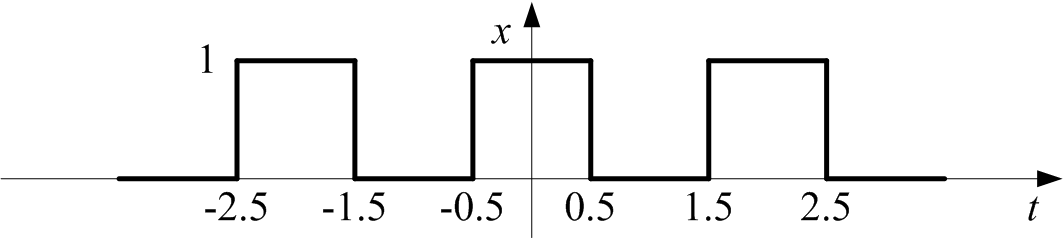
\includegraphics[height=2cm]{4.1.5-1.png}
\end{figure}
\end{example}

易得$T=2,\omega _0=\pi ,\omega _n=n\pi $,计算傅里叶系数:
\begin{align*}
C_0&=\frac{1}{T}\int_{-\frac{T}{2}}^{\frac{T}{2}}{x\left( t \right) dt}=\frac{1}{2}\int_{-1}^1{x\left( t \right) dt}=\frac{1}{2}\int_{-0.5}^{0.5}{dt}=\frac{1}{2} \\
C_n&=\frac{1}{T}\int_{-\frac{T}{2}}^{\frac{T}{2}}{x\left( t \right) e^{-i\omega _nt}dt}=\frac{1}{2}\int_{-0.5}^{0.5}{e^{-in\pi t}dt} =\frac{i}{2n\pi}\left( e^{-\frac{in\pi}{2}}-e^{\frac{in\pi}{2}} \right) \\
&=\frac{i}{2n\pi}\left[ \cos \left( -\frac{n\pi}{2} \right) +i\sin \left( -\frac{n\pi}{2} \right) -\cos \left( \frac{n\pi}{2} \right) -i\sin \left( \frac{n\pi}{2} \right) \right] \\
&=\frac{1}{n\pi}\sin \left( \frac{n\pi}{2} \right)
\end{align*}
由于$\sin \left( \frac{n\pi}{2} \right) =0,n=0,\pm 2,\pm 4,\cdots $,所以跳过偶数以减小计算量,得到最终的傅里叶级数:
\[
x\left( t \right) =C_0+\sum_{n=\pm 1,odd}^{\pm \infty}{\left[ C_n\cdot e^{in\pi t} \right]}=\frac{1}{2}+\sum_{n=1,odd}^{+\infty}{\left[ 2\cdot \frac{\sin \left( n\pi /2 \right)}{n\pi}\cdot \cos \left( n\pi t \right) \right]}
\]
用Python分别对累加至3、8、20、100次谐波的傅里叶级数作图如下,谐波叠加越多,越能近似原信号。
\begin{figure}[h]
\centering
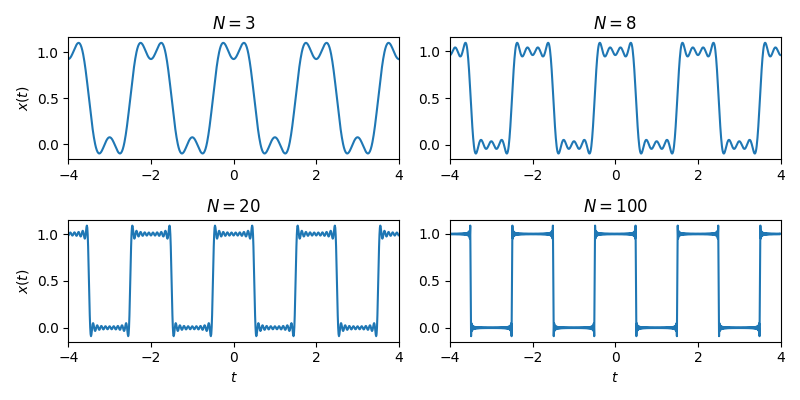
\includegraphics[height=5cm]{4.1.5-2.png}
\end{figure}

\begin{python}
t  = np.arange(-4, 4, 0.01)
x1 = np.full_like(t, 0.5, dtype=np.float32)
N = 3
for n in range(1,N+1,2):
    x1 += 2/n/np.pi * np.sin(n*np.pi/2) * np.cos(n*np.pi*t)
    pass

axs[0][0].plot(t, x1)
\end{python}

\begin{tcolorbox}
由于时域方波有不连续点,不满足狄利克雷收敛条件,所以在这些间断点,傅里叶级数和原函数有9\%的误差,称为{\bf Gibbs现象}。
\end{tcolorbox}

~

\begin{example}
假设如下图信号,求傅里叶级数,当$T=2,a=0.5$时,用Python作图验证。
\begin{figure}[h]
\centering
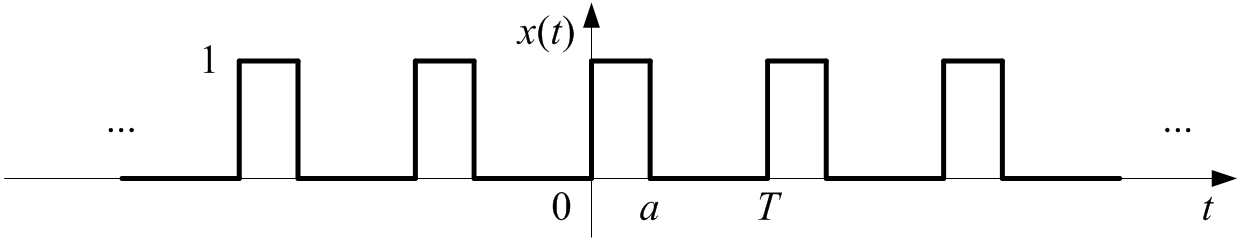
\includegraphics[height=2cm]{4.1.5-3.png}
\end{figure}
\end{example}

计算傅里叶系数:
\begin{align*}
&C_0=\frac{1}{T}\int_{-\frac{T}{2}}^{\frac{T}{2}}{x\left( t \right) dt}=\frac{1}{T}\int_0^a{dt}=\frac{a}{T} \\
&C_n=\frac{1}{T}\int_{-\frac{T}{2}}^{\frac{T}{2}}{x\left( t \right) e^{-i\omega _nt}dt}=\frac{1}{T}\int_0^a{e^{-in\frac{2\pi}{T}t}dt} =\frac{i}{2n\pi}\left( e^{-\frac{i2an\pi}{T}}-1 \right)
\end{align*}
得傅里叶级数:
\[
x\left( t \right) =C_0+\sum_{n=\pm 1}^{\pm \infty}{\left[ C_n\cdot e^{in\frac{2\pi}{T}t} \right]}=\frac{a}{T}+\sum_{n=1}^{+\infty}{\frac{\sin \frac{2n\pi t}{T}-\sin \frac{2n\pi \left( t-a \right)}{T}}{n\pi}}
\]
\begin{figure}[h]
\centering
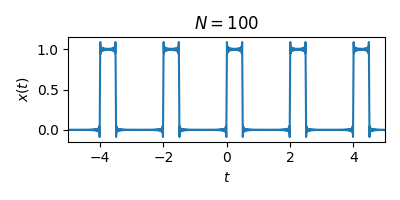
\includegraphics[height=3cm]{4.1.5-4.png}
\end{figure}

~

\begin{example}
设如下图信号,求傅里叶级数,用Python作图验证。
\begin{figure}[h]
\centering
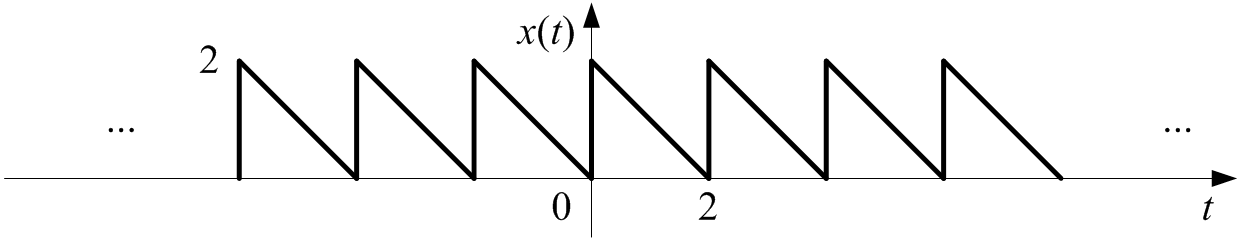
\includegraphics[height=2cm]{4.1.5-5.png}
\end{figure}
\end{example}

显然,信号有$x\left( t \right) =2-t,T=2$,计算傅里叶系数:
\begin{align*}
&C_0=\frac{1}{T}\int_{-\frac{T}{2}}^{\frac{T}{2}}{x\left( t \right) dt}=\frac{1}{2}\int_0^2{\left( 2-t \right) dt}=1 \\
&C_n=\frac{1}{T}\int_{-\frac{T}{2}}^{\frac{T}{2}}{x\left( t \right) e^{-i\omega _nt}dt}=\frac{1}{2}\int_0^2{\left( 2-t \right) e^{-i\omega _nt}dt}=\frac{1-i2\omega _n-e^{-i2\omega _n}}{2{\omega _n}^2}
\end{align*}
得傅里叶级数:
\begin{align*}
x\left( t \right) &=C_0+\sum_{n=\pm 1}^{\pm \infty}{\left[ C_n\cdot e^{in\omega _nt} \right]} \\
&=1+\sum_{n=1}^{+\infty}{\frac{\cos \left( n\pi t \right) +2n\pi \sin \left( n\pi t \right) -\cos \left( n\pi \left( t-2 \right) \right)}{\left( n\pi \right) ^2}}
\end{align*}
\begin{figure}[h]
\centering
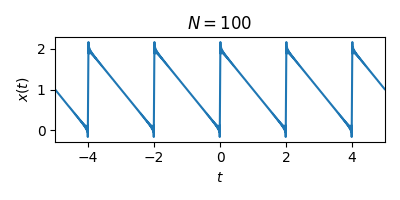
\includegraphics[height=3cm]{4.1.5-6.png}
\end{figure}




